\documentclass[twoside]{book}

% Packages required by doxygen
\usepackage{fixltx2e}
\usepackage{calc}
\usepackage{doxygen}
\usepackage[export]{adjustbox} % also loads graphicx
\usepackage{graphicx}
\usepackage[utf8]{inputenc}
\usepackage{makeidx}
\usepackage{multicol}
\usepackage{multirow}
\PassOptionsToPackage{warn}{textcomp}
\usepackage{textcomp}
\usepackage[nointegrals]{wasysym}
\usepackage[table]{xcolor}

% NLS support packages
Portuguese
% Font selection
\usepackage[T1]{fontenc}
\usepackage[scaled=.90]{helvet}
\usepackage{courier}
\usepackage{amssymb}
\usepackage{sectsty}
\renewcommand{\familydefault}{\sfdefault}
\allsectionsfont{%
  \fontseries{bc}\selectfont%
  \color{darkgray}%
}
\renewcommand{\DoxyLabelFont}{%
  \fontseries{bc}\selectfont%
  \color{darkgray}%
}
\newcommand{\+}{\discretionary{\mbox{\scriptsize$\hookleftarrow$}}{}{}}

% Page & text layout
\usepackage{geometry}
\geometry{%
  a4paper,%
  top=2.5cm,%
  bottom=2.5cm,%
  left=2.5cm,%
  right=2.5cm%
}
\tolerance=750
\hfuzz=15pt
\hbadness=750
\setlength{\emergencystretch}{15pt}
\setlength{\parindent}{0cm}
\setlength{\parskip}{3ex plus 2ex minus 2ex}
\makeatletter
\renewcommand{\paragraph}{%
  \@startsection{paragraph}{4}{0ex}{-1.0ex}{1.0ex}{%
    \normalfont\normalsize\bfseries\SS@parafont%
  }%
}
\renewcommand{\subparagraph}{%
  \@startsection{subparagraph}{5}{0ex}{-1.0ex}{1.0ex}{%
    \normalfont\normalsize\bfseries\SS@subparafont%
  }%
}
\makeatother

% Headers & footers
\usepackage{fancyhdr}
\pagestyle{fancyplain}
\fancyhead[LE]{\fancyplain{}{\bfseries\thepage}}
\fancyhead[CE]{\fancyplain{}{}}
\fancyhead[RE]{\fancyplain{}{\bfseries\leftmark}}
\fancyhead[LO]{\fancyplain{}{\bfseries\rightmark}}
\fancyhead[CO]{\fancyplain{}{}}
\fancyhead[RO]{\fancyplain{}{\bfseries\thepage}}
\fancyfoot[LE]{\fancyplain{}{}}
\fancyfoot[CE]{\fancyplain{}{}}
\fancyfoot[RE]{\fancyplain{}{\bfseries\scriptsize Gerado por Doxygen }}
\fancyfoot[LO]{\fancyplain{}{\bfseries\scriptsize Gerado por Doxygen }}
\fancyfoot[CO]{\fancyplain{}{}}
\fancyfoot[RO]{\fancyplain{}{}}
\renewcommand{\footrulewidth}{0.4pt}
\renewcommand{\chaptermark}[1]{%
  \markboth{#1}{}%
}
\renewcommand{\sectionmark}[1]{%
  \markright{\thesection\ #1}%
}

% Indices & bibliography
\usepackage{natbib}
\usepackage[titles]{tocloft}
\setcounter{tocdepth}{3}
\setcounter{secnumdepth}{5}
\makeindex

% Hyperlinks (required, but should be loaded last)
\usepackage{ifpdf}
\ifpdf
  \usepackage[pdftex,pagebackref=true]{hyperref}
\else
  \usepackage[ps2pdf,pagebackref=true]{hyperref}
\fi
\hypersetup{%
  colorlinks=true,%
  linkcolor=blue,%
  citecolor=blue,%
  unicode%
}

% Custom commands
\newcommand{\clearemptydoublepage}{%
  \newpage{\pagestyle{empty}\cleardoublepage}%
}

\usepackage{caption}
\captionsetup{labelsep=space,justification=centering,font={bf},singlelinecheck=off,skip=4pt,position=top}

%===== C O N T E N T S =====

\begin{document}

% Titlepage & ToC
\hypersetup{pageanchor=false,
             bookmarksnumbered=true,
             pdfencoding=unicode
            }
\pagenumbering{alph}
\begin{titlepage}
\vspace*{7cm}
\begin{center}%
{\Large My Project }\\
\vspace*{1cm}
{\large Gerado por Doxygen 1.8.13}\\
\end{center}
\end{titlepage}
\clearemptydoublepage
\pagenumbering{roman}
\tableofcontents
\clearemptydoublepage
\pagenumbering{arabic}
\hypersetup{pageanchor=true}

%--- Begin generated contents ---
\chapter{Contador de Veículos}
\label{index}\hypertarget{index}{}\hypertarget{index_intro_sec}{}\section{Introdução}\label{index_intro_sec}
Esse projeto consiste em um sistema capaz de contar o número de veículos que estão de passagem em uma rodovia com a utilização de técnicas aprendidas em Processamentos Digitais de Sinais\hypertarget{index_install_sec}{}\section{Execução}\label{index_install_sec}
Executar os comandos na pasta base do projeto\+: ~\newline
 g++ -\/o main $\ast$.cpp {\ttfamily pkg-\/config -\/-\/cflags -\/-\/libs opencv} ~\newline
 ./main 
\chapter{Vehicle-\/\+Counter-\/\+Open\+C\+V-\/\+Cpp}
\label{md__r_e_a_d_m_e}
\Hypertarget{md__r_e_a_d_m_e}
\input{md__r_e_a_d_m_e}
\chapter{Índice dos componentes}
\section{Lista de componentes}
Lista de classes, estruturas, uniões e interfaces com uma breve descrição\+:\begin{DoxyCompactList}
\item\contentsline{section}{\hyperlink{class_blob}{Blob} }{\pageref{class_blob}}{}
\end{DoxyCompactList}

\chapter{Índice dos ficheiros}
\section{Lista de ficheiros}
Lista de todos os ficheiros com uma breve descrição\+:\begin{DoxyCompactList}
\item\contentsline{section}{\hyperlink{_blob_8cpp}{Blob.\+cpp} }{\pageref{_blob_8cpp}}{}
\item\contentsline{section}{\hyperlink{_blob_8h}{Blob.\+h} }{\pageref{_blob_8h}}{}
\item\contentsline{section}{\hyperlink{_main_8cpp}{Main.\+cpp} }{\pageref{_main_8cpp}}{}
\end{DoxyCompactList}

\chapter{Documentação da classe}
\hypertarget{class_blob}{}\section{Referência à classe Blob}
\label{class_blob}\index{Blob@{Blob}}


{\ttfamily \#include $<$Blob.\+h$>$}



Diagrama de colaboração para Blob\+:
\nopagebreak
\begin{figure}[H]
\begin{center}
\leavevmode
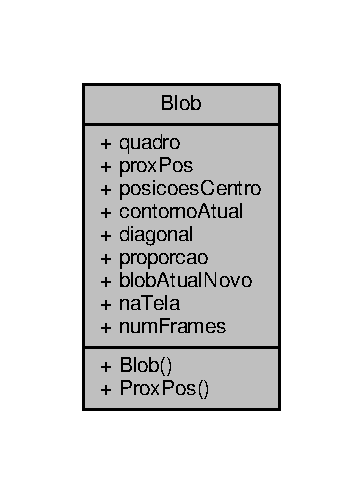
\includegraphics[width=174pt]{class_blob__coll__graph}
\end{center}
\end{figure}
\subsection*{Membros públicos}
\begin{DoxyCompactItemize}
\item 
\hyperlink{class_blob_af61bf71a4f486a4eeba6165bbfdbb8f6}{Blob} (vector$<$ Point $>$ contorno)
\item 
void \hyperlink{class_blob_afbea7ea42d7e01e4d84c799d5fd7e8a5}{Prox\+Pos} (void)
\end{DoxyCompactItemize}
\subsection*{Atributos Públicos}
\begin{DoxyCompactItemize}
\item 
Rect \hyperlink{class_blob_aa6387723adb0b9bc5972cf68cc85f4b3}{quadro}
\item 
Point \hyperlink{class_blob_ad4eeb7d2aa4ef4f6c6e038737ce41043}{prox\+Pos}
\item 
vector$<$ Point $>$ \hyperlink{class_blob_a07f56ca5b367f2a9b15622d92e2c671a}{posicoes\+Centro}
\item 
vector$<$ Point $>$ \hyperlink{class_blob_a83d705f2b426be288d87c6f606175889}{contorno\+Atual}
\item 
double \hyperlink{class_blob_ad77546934e684be45fa6d12d8370d0c7}{diagonal}
\item 
double \hyperlink{class_blob_a0e1f64cf95a07d948728f9e00d1feec1}{proporcao}
\item 
bool \hyperlink{class_blob_a121b1af88b7c0752403f6eca92ab2150}{blob\+Atual\+Novo}
\item 
bool \hyperlink{class_blob_a57b76134e44f731fdb2afcf85de066c4}{na\+Tela}
\item 
int \hyperlink{class_blob_a3c6b8107db4ef7269ad117f1120a69e3}{num\+Frames}
\end{DoxyCompactItemize}


\subsection{Documentação dos Construtores \& Destrutor}
\mbox{\Hypertarget{class_blob_af61bf71a4f486a4eeba6165bbfdbb8f6}\label{class_blob_af61bf71a4f486a4eeba6165bbfdbb8f6}} 
\index{Blob@{Blob}!Blob@{Blob}}
\index{Blob@{Blob}!Blob@{Blob}}
\subsubsection{\texorpdfstring{Blob()}{Blob()}}
{\footnotesize\ttfamily Blob\+::\+Blob (\begin{DoxyParamCaption}\item[{vector$<$ Point $>$}]{contorno }\end{DoxyParamCaption})}

Número consecutivo de frames sem parecer com o blob

Inicializa os parâmetros do blob Calcula o centro do blob

Calcula a diagonal do quadro do blob

Calcula a proporção do quadro do blob

Define que o blob está na tela e é atual/novo 

\subsection{Documentação dos métodos}
\mbox{\Hypertarget{class_blob_afbea7ea42d7e01e4d84c799d5fd7e8a5}\label{class_blob_afbea7ea42d7e01e4d84c799d5fd7e8a5}} 
\index{Blob@{Blob}!Prox\+Pos@{Prox\+Pos}}
\index{Prox\+Pos@{Prox\+Pos}!Blob@{Blob}}
\subsubsection{\texorpdfstring{Prox\+Pos()}{ProxPos()}}
{\footnotesize\ttfamily void Blob\+::\+Prox\+Pos (\begin{DoxyParamCaption}\item[{void}]{ }\end{DoxyParamCaption})}

Calcula a próxima posição do centro do blob 

\subsection{Documentação dos dados membro}
\mbox{\Hypertarget{class_blob_a121b1af88b7c0752403f6eca92ab2150}\label{class_blob_a121b1af88b7c0752403f6eca92ab2150}} 
\index{Blob@{Blob}!blob\+Atual\+Novo@{blob\+Atual\+Novo}}
\index{blob\+Atual\+Novo@{blob\+Atual\+Novo}!Blob@{Blob}}
\subsubsection{\texorpdfstring{blob\+Atual\+Novo}{blobAtualNovo}}
{\footnotesize\ttfamily bool Blob\+::blob\+Atual\+Novo}

Proporção do quadro do blob \mbox{\Hypertarget{class_blob_a83d705f2b426be288d87c6f606175889}\label{class_blob_a83d705f2b426be288d87c6f606175889}} 
\index{Blob@{Blob}!contorno\+Atual@{contorno\+Atual}}
\index{contorno\+Atual@{contorno\+Atual}!Blob@{Blob}}
\subsubsection{\texorpdfstring{contorno\+Atual}{contornoAtual}}
{\footnotesize\ttfamily vector$<$Point$>$ Blob\+::contorno\+Atual}

Coordenadas do centro do blob \mbox{\Hypertarget{class_blob_ad77546934e684be45fa6d12d8370d0c7}\label{class_blob_ad77546934e684be45fa6d12d8370d0c7}} 
\index{Blob@{Blob}!diagonal@{diagonal}}
\index{diagonal@{diagonal}!Blob@{Blob}}
\subsubsection{\texorpdfstring{diagonal}{diagonal}}
{\footnotesize\ttfamily double Blob\+::diagonal}

Contorno do blob \mbox{\Hypertarget{class_blob_a57b76134e44f731fdb2afcf85de066c4}\label{class_blob_a57b76134e44f731fdb2afcf85de066c4}} 
\index{Blob@{Blob}!na\+Tela@{na\+Tela}}
\index{na\+Tela@{na\+Tela}!Blob@{Blob}}
\subsubsection{\texorpdfstring{na\+Tela}{naTela}}
{\footnotesize\ttfamily bool Blob\+::na\+Tela}

Verifica se o blob é atual/novo ou antigo \mbox{\Hypertarget{class_blob_a3c6b8107db4ef7269ad117f1120a69e3}\label{class_blob_a3c6b8107db4ef7269ad117f1120a69e3}} 
\index{Blob@{Blob}!num\+Frames@{num\+Frames}}
\index{num\+Frames@{num\+Frames}!Blob@{Blob}}
\subsubsection{\texorpdfstring{num\+Frames}{numFrames}}
{\footnotesize\ttfamily int Blob\+::num\+Frames}

Verifica se o blob ainda está na tela \mbox{\Hypertarget{class_blob_a07f56ca5b367f2a9b15622d92e2c671a}\label{class_blob_a07f56ca5b367f2a9b15622d92e2c671a}} 
\index{Blob@{Blob}!posicoes\+Centro@{posicoes\+Centro}}
\index{posicoes\+Centro@{posicoes\+Centro}!Blob@{Blob}}
\subsubsection{\texorpdfstring{posicoes\+Centro}{posicoesCentro}}
{\footnotesize\ttfamily vector$<$Point$>$ Blob\+::posicoes\+Centro}

Próxima posição do centro do blob \mbox{\Hypertarget{class_blob_a0e1f64cf95a07d948728f9e00d1feec1}\label{class_blob_a0e1f64cf95a07d948728f9e00d1feec1}} 
\index{Blob@{Blob}!proporcao@{proporcao}}
\index{proporcao@{proporcao}!Blob@{Blob}}
\subsubsection{\texorpdfstring{proporcao}{proporcao}}
{\footnotesize\ttfamily double Blob\+::proporcao}

Diagonal do quadro do blob \mbox{\Hypertarget{class_blob_ad4eeb7d2aa4ef4f6c6e038737ce41043}\label{class_blob_ad4eeb7d2aa4ef4f6c6e038737ce41043}} 
\index{Blob@{Blob}!prox\+Pos@{prox\+Pos}}
\index{prox\+Pos@{prox\+Pos}!Blob@{Blob}}
\subsubsection{\texorpdfstring{prox\+Pos}{proxPos}}
{\footnotesize\ttfamily Point Blob\+::prox\+Pos}

Contorno retangular do blob \mbox{\Hypertarget{class_blob_aa6387723adb0b9bc5972cf68cc85f4b3}\label{class_blob_aa6387723adb0b9bc5972cf68cc85f4b3}} 
\index{Blob@{Blob}!quadro@{quadro}}
\index{quadro@{quadro}!Blob@{Blob}}
\subsubsection{\texorpdfstring{quadro}{quadro}}
{\footnotesize\ttfamily Rect Blob\+::quadro}



A documentação para esta classe foi gerada a partir dos seguintes ficheiros\+:\begin{DoxyCompactItemize}
\item 
\hyperlink{_blob_8h}{Blob.\+h}\item 
\hyperlink{_blob_8cpp}{Blob.\+cpp}\end{DoxyCompactItemize}

\chapter{Documentação do ficheiro}
\hypertarget{_blob_8cpp}{}\section{Referência ao ficheiro Blob.\+cpp}
\label{_blob_8cpp}\index{Blob.\+cpp@{Blob.\+cpp}}
{\ttfamily \#include \char`\"{}Blob.\+h\char`\"{}}\newline
Diagrama de dependências de inclusão para Blob.\+cpp\+:
\nopagebreak
\begin{figure}[H]
\begin{center}
\leavevmode
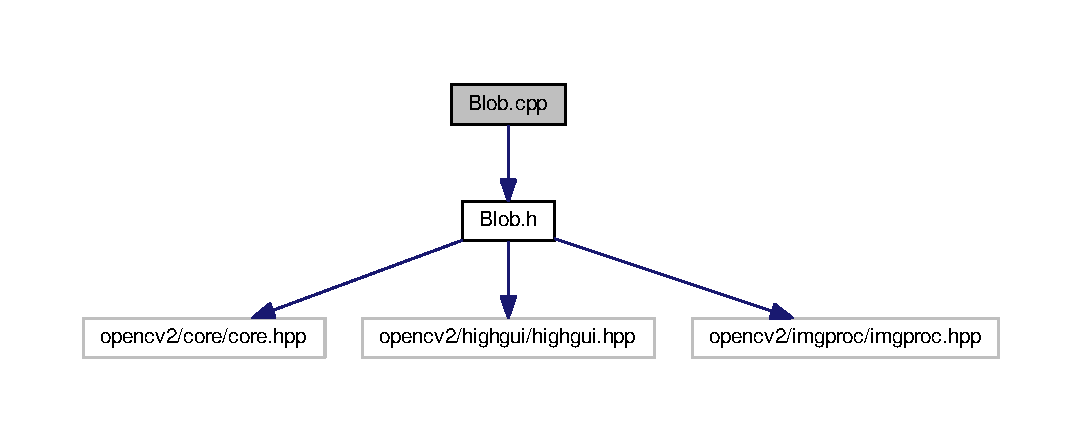
\includegraphics[width=350pt]{_blob_8cpp__incl}
\end{center}
\end{figure}

\hypertarget{_blob_8h}{}\section{Referência ao ficheiro Blob.\+h}
\label{_blob_8h}\index{Blob.\+h@{Blob.\+h}}
{\ttfamily \#include $<$opencv2/core/core.\+hpp$>$}\newline
{\ttfamily \#include $<$opencv2/highgui/highgui.\+hpp$>$}\newline
{\ttfamily \#include $<$opencv2/imgproc/imgproc.\+hpp$>$}\newline
Diagrama de dependências de inclusão para Blob.\+h\+:
\nopagebreak
\begin{figure}[H]
\begin{center}
\leavevmode
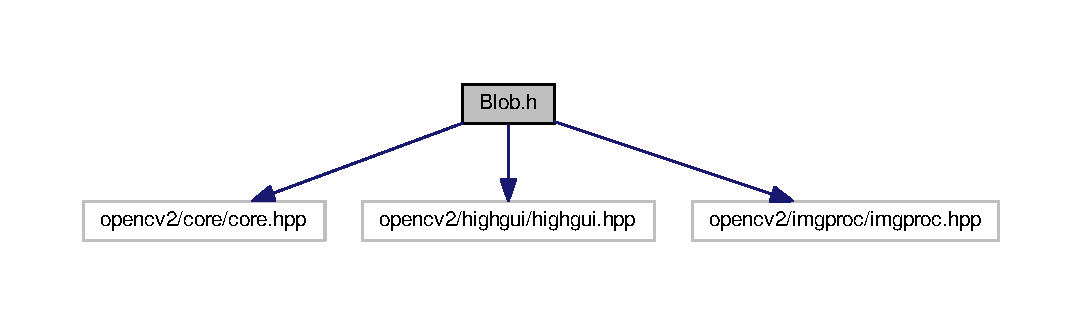
\includegraphics[width=350pt]{_blob_8h__incl}
\end{center}
\end{figure}
Este grafo mostra quais são os ficheiros que incluem directamente ou indirectamente este ficheiro\+:
\nopagebreak
\begin{figure}[H]
\begin{center}
\leavevmode
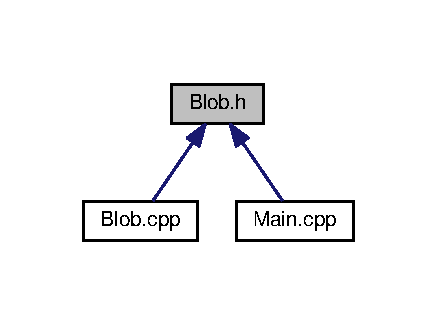
\includegraphics[width=210pt]{_blob_8h__dep__incl}
\end{center}
\end{figure}
\subsection*{Componentes}
\begin{DoxyCompactItemize}
\item 
class \hyperlink{class_blob}{Blob}
\end{DoxyCompactItemize}

\hypertarget{_main_8cpp}{}\section{Referência ao ficheiro Main.\+cpp}
\label{_main_8cpp}\index{Main.\+cpp@{Main.\+cpp}}
{\ttfamily \#include $<$fstream$>$}\newline
{\ttfamily \#include $<$iomanip$>$}\newline
{\ttfamily \#include $<$iostream$>$}\newline
{\ttfamily \#include $<$opencv2/core/core.\+hpp$>$}\newline
{\ttfamily \#include $<$opencv2/highgui/highgui.\+hpp$>$}\newline
{\ttfamily \#include $<$opencv2/imgproc/imgproc.\+hpp$>$}\newline
{\ttfamily \#include $<$string$>$}\newline
{\ttfamily \#include \char`\"{}Blob.\+h\char`\"{}}\newline
Diagrama de dependências de inclusão para Main.\+cpp\+:
\nopagebreak
\begin{figure}[H]
\begin{center}
\leavevmode
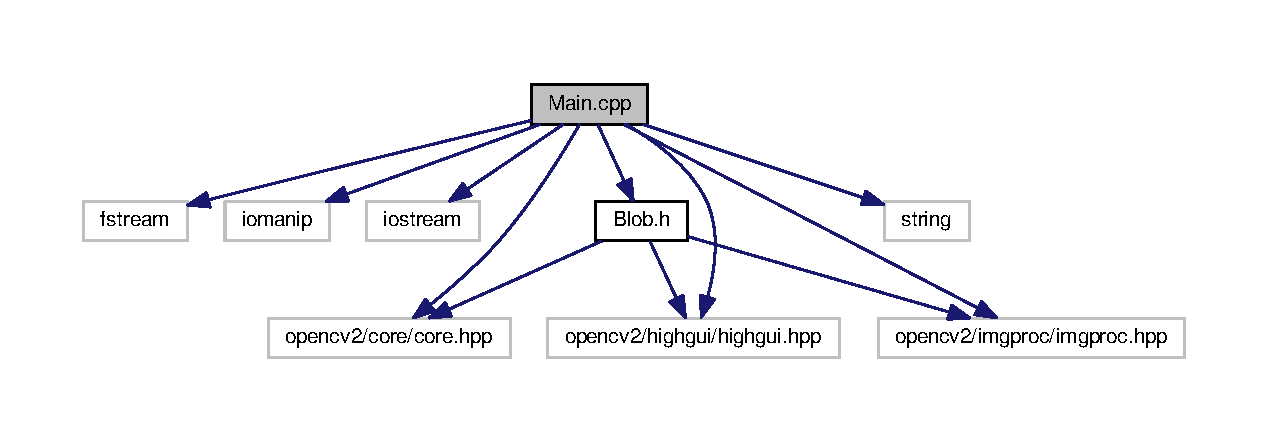
\includegraphics[width=350pt]{_main_8cpp__incl}
\end{center}
\end{figure}
\subsection*{Funções}
\begin{DoxyCompactItemize}
\item 
double \hyperlink{_main_8cpp_af393771749f2513a141d946bb885291b}{dist\+Pontos} (Point ponto1, Point ponto2)
\item 
void \hyperlink{_main_8cpp_afd251a63f3d03c2563a1f1dcf0ccb6f0}{insere\+Blob} (\hyperlink{class_blob}{Blob} \&blob\+Atual, vector$<$ \hyperlink{class_blob}{Blob} $>$ \&blobs\+Existentes, int \&int\+Index)
\item 
void \hyperlink{_main_8cpp_a71c7b1ac1ca05b2e298a38fa1f7e58f8}{novo\+Blob} (\hyperlink{class_blob}{Blob} \&blob\+Atual, vector$<$ \hyperlink{class_blob}{Blob} $>$ \&blobs\+Existentes)
\item 
void \hyperlink{_main_8cpp_a3b43a4786c55005af285428e7c7ced87}{verifica\+Blob} (vector$<$ \hyperlink{class_blob}{Blob} $>$ \&blobs\+Existentes, vector$<$ \hyperlink{class_blob}{Blob} $>$ \&blobs\+Atuais)
\item 
void \hyperlink{_main_8cpp_ada3c309241ca0406bdf3a8cce848abf2}{Contorno} (Size image\+Size, vector$<$ vector$<$ Point $>$$>$ contornos, string str\+Image\+Name)
\item 
void \hyperlink{_main_8cpp_a08a385c14c747c894052ff8664a51dff}{Contorno} (Size image\+Size, vector$<$ \hyperlink{class_blob}{Blob} $>$ blobs\+Existentes, string str\+Image\+Name)
\item 
bool \hyperlink{_main_8cpp_a69dab197c810eaf3e966b71fd45b8df3}{cruzou\+Linha\+Dir} (vector$<$ \hyperlink{class_blob}{Blob} $>$ \&blobs\+Existentes, int \&linha\+Hor, int \&\hyperlink{_main_8cpp_a58d02c40e7b027e0b1ff6ce88c63280e}{cont\+Dir})
\item 
bool \hyperlink{_main_8cpp_a6c2c44c0ed121fc428f0f2be7d870f37}{cruzou\+Linha\+Esq} (vector$<$ \hyperlink{class_blob}{Blob} $>$ \&blobs\+Existentes, int \&linha\+Hor, int \&\hyperlink{_main_8cpp_a6bd1388b3554788f7d8d2019b2e00303}{cont\+Esq})
\item 
void \hyperlink{_main_8cpp_a4d5709a14b312373c1bebc1e0cc51479}{blob\+Info} (vector$<$ \hyperlink{class_blob}{Blob} $>$ \&blobs\+Existentes, Mat \&clone\+Frame2)
\item 
void \hyperlink{_main_8cpp_a1ac43d4e5e9f9024d51d4df35879a7e3}{contador} (int \&\hyperlink{_main_8cpp_a58d02c40e7b027e0b1ff6ce88c63280e}{cont\+Dir}, Mat \&clone\+Frame2)
\item 
int \hyperlink{_main_8cpp_a840291bc02cba5474a4cb46a9b9566fe}{main} (void)
\end{DoxyCompactItemize}
\subsection*{Variáveis}
\begin{DoxyCompactItemize}
\item 
const Scalar \hyperlink{_main_8cpp_a5f80550661781105dac995103754a262}{P\+R\+E\+TO} = Scalar(0.\+0, 0.\+0, 0.\+0)
\item 
const Scalar \hyperlink{_main_8cpp_a7c4a0519bc3e090ee4e3831391a9e018}{B\+R\+A\+N\+CO} = Scalar(255.\+0, 255.\+0, 255.\+0)
\item 
const Scalar \hyperlink{_main_8cpp_a7b2cb89c87c76a1d832ef7ed097d9505}{A\+M\+A\+R\+E\+LO} = Scalar(0.\+0, 255.\+0, 255.\+0)
\item 
const Scalar \hyperlink{_main_8cpp_aba06b79f5f073991c8a0afa7ebf9f534}{V\+E\+R\+DE} = Scalar(0.\+0, 200.\+0, 0.\+0)
\item 
const Scalar \hyperlink{_main_8cpp_a4d72d63fede13ee55603d480e2c28fd8}{V\+E\+R\+M\+E\+L\+HO} = Scalar(0.\+0, 0.\+0, 255.\+0)
\item 
int \hyperlink{_main_8cpp_a6bd1388b3554788f7d8d2019b2e00303}{cont\+Esq} = 0
\item 
int \hyperlink{_main_8cpp_a58d02c40e7b027e0b1ff6ce88c63280e}{cont\+Dir} = 0
\end{DoxyCompactItemize}


\subsection{Documentação das funções}
\mbox{\Hypertarget{_main_8cpp_a4d5709a14b312373c1bebc1e0cc51479}\label{_main_8cpp_a4d5709a14b312373c1bebc1e0cc51479}} 
\index{Main.\+cpp@{Main.\+cpp}!blob\+Info@{blob\+Info}}
\index{blob\+Info@{blob\+Info}!Main.\+cpp@{Main.\+cpp}}
\subsubsection{\texorpdfstring{blob\+Info()}{blobInfo()}}
{\footnotesize\ttfamily void blob\+Info (\begin{DoxyParamCaption}\item[{vector$<$ \hyperlink{class_blob}{Blob} $>$ \&}]{blobs\+Existentes,  }\item[{Mat \&}]{clone\+Frame2 }\end{DoxyParamCaption})}

Imprime as informações do blob na tela Parâmetros da fonte Este é o diagrama das funções que utilizam esta função\+:
\nopagebreak
\begin{figure}[H]
\begin{center}
\leavevmode
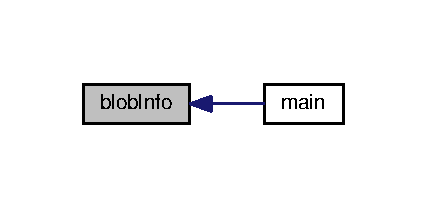
\includegraphics[width=205pt]{_main_8cpp_a4d5709a14b312373c1bebc1e0cc51479_icgraph}
\end{center}
\end{figure}
\mbox{\Hypertarget{_main_8cpp_a1ac43d4e5e9f9024d51d4df35879a7e3}\label{_main_8cpp_a1ac43d4e5e9f9024d51d4df35879a7e3}} 
\index{Main.\+cpp@{Main.\+cpp}!contador@{contador}}
\index{contador@{contador}!Main.\+cpp@{Main.\+cpp}}
\subsubsection{\texorpdfstring{contador()}{contador()}}
{\footnotesize\ttfamily void contador (\begin{DoxyParamCaption}\item[{int \&}]{cont\+Dir,  }\item[{Mat \&}]{clone\+Frame2 }\end{DoxyParamCaption})}

Imprime o contador na imagem Contador da via direita

Contador da via esquerda Este é o diagrama das funções que utilizam esta função\+:
\nopagebreak
\begin{figure}[H]
\begin{center}
\leavevmode
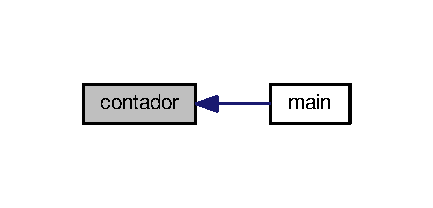
\includegraphics[width=208pt]{_main_8cpp_a1ac43d4e5e9f9024d51d4df35879a7e3_icgraph}
\end{center}
\end{figure}
\mbox{\Hypertarget{_main_8cpp_ada3c309241ca0406bdf3a8cce848abf2}\label{_main_8cpp_ada3c309241ca0406bdf3a8cce848abf2}} 
\index{Main.\+cpp@{Main.\+cpp}!Contorno@{Contorno}}
\index{Contorno@{Contorno}!Main.\+cpp@{Main.\+cpp}}
\subsubsection{\texorpdfstring{Contorno()}{Contorno()}\hspace{0.1cm}{\footnotesize\ttfamily [1/2]}}
{\footnotesize\ttfamily void Contorno (\begin{DoxyParamCaption}\item[{Size}]{image\+Size,  }\item[{vector$<$ vector$<$ Point $>$$>$}]{contornos,  }\item[{string}]{str\+Image\+Name }\end{DoxyParamCaption})}

Desenha o contorno dos blobs Este é o diagrama das funções que utilizam esta função\+:
\nopagebreak
\begin{figure}[H]
\begin{center}
\leavevmode
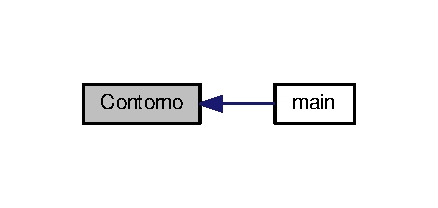
\includegraphics[width=210pt]{_main_8cpp_ada3c309241ca0406bdf3a8cce848abf2_icgraph}
\end{center}
\end{figure}
\mbox{\Hypertarget{_main_8cpp_a08a385c14c747c894052ff8664a51dff}\label{_main_8cpp_a08a385c14c747c894052ff8664a51dff}} 
\index{Main.\+cpp@{Main.\+cpp}!Contorno@{Contorno}}
\index{Contorno@{Contorno}!Main.\+cpp@{Main.\+cpp}}
\subsubsection{\texorpdfstring{Contorno()}{Contorno()}\hspace{0.1cm}{\footnotesize\ttfamily [2/2]}}
{\footnotesize\ttfamily void Contorno (\begin{DoxyParamCaption}\item[{Size}]{image\+Size,  }\item[{vector$<$ \hyperlink{class_blob}{Blob} $>$}]{blobs\+Existentes,  }\item[{string}]{str\+Image\+Name }\end{DoxyParamCaption})}

Desenha o contorno dos blobs \mbox{\Hypertarget{_main_8cpp_a69dab197c810eaf3e966b71fd45b8df3}\label{_main_8cpp_a69dab197c810eaf3e966b71fd45b8df3}} 
\index{Main.\+cpp@{Main.\+cpp}!cruzou\+Linha\+Dir@{cruzou\+Linha\+Dir}}
\index{cruzou\+Linha\+Dir@{cruzou\+Linha\+Dir}!Main.\+cpp@{Main.\+cpp}}
\subsubsection{\texorpdfstring{cruzou\+Linha\+Dir()}{cruzouLinhaDir()}}
{\footnotesize\ttfamily bool cruzou\+Linha\+Dir (\begin{DoxyParamCaption}\item[{vector$<$ \hyperlink{class_blob}{Blob} $>$ \&}]{blobs\+Existentes,  }\item[{int \&}]{linha\+Hor,  }\item[{int \&}]{cont\+Dir }\end{DoxyParamCaption})}

Verifica se o veículo cruzou a linha da direita Verifica se pelo menos 1 blob cruzou a linha

Índice do frame anterior

Índice do frame atual

Se um blob cruzou a linha, incrementa o contador da via direita Este é o diagrama das funções que utilizam esta função\+:
\nopagebreak
\begin{figure}[H]
\begin{center}
\leavevmode
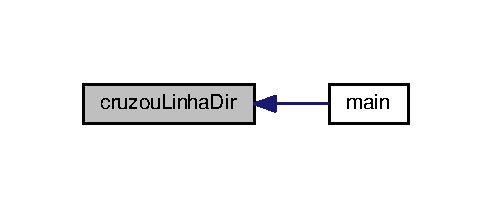
\includegraphics[width=236pt]{_main_8cpp_a69dab197c810eaf3e966b71fd45b8df3_icgraph}
\end{center}
\end{figure}
\mbox{\Hypertarget{_main_8cpp_a6c2c44c0ed121fc428f0f2be7d870f37}\label{_main_8cpp_a6c2c44c0ed121fc428f0f2be7d870f37}} 
\index{Main.\+cpp@{Main.\+cpp}!cruzou\+Linha\+Esq@{cruzou\+Linha\+Esq}}
\index{cruzou\+Linha\+Esq@{cruzou\+Linha\+Esq}!Main.\+cpp@{Main.\+cpp}}
\subsubsection{\texorpdfstring{cruzou\+Linha\+Esq()}{cruzouLinhaEsq()}}
{\footnotesize\ttfamily bool cruzou\+Linha\+Esq (\begin{DoxyParamCaption}\item[{vector$<$ \hyperlink{class_blob}{Blob} $>$ \&}]{blobs\+Existentes,  }\item[{int \&}]{linha\+Hor,  }\item[{int \&}]{cont\+Esq }\end{DoxyParamCaption})}

Verifica se o veículo cruzou a linha da esquerda Verifica se pelo menos 1 blob cruzou a linha

Índice do frame anterior

Índice do frame atual

Se um blob cruzou a linha, incrementa o contador da via esquerda Este é o diagrama das funções que utilizam esta função\+:
\nopagebreak
\begin{figure}[H]
\begin{center}
\leavevmode
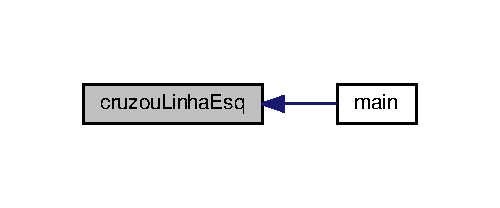
\includegraphics[width=240pt]{_main_8cpp_a6c2c44c0ed121fc428f0f2be7d870f37_icgraph}
\end{center}
\end{figure}
\mbox{\Hypertarget{_main_8cpp_af393771749f2513a141d946bb885291b}\label{_main_8cpp_af393771749f2513a141d946bb885291b}} 
\index{Main.\+cpp@{Main.\+cpp}!dist\+Pontos@{dist\+Pontos}}
\index{dist\+Pontos@{dist\+Pontos}!Main.\+cpp@{Main.\+cpp}}
\subsubsection{\texorpdfstring{dist\+Pontos()}{distPontos()}}
{\footnotesize\ttfamily double dist\+Pontos (\begin{DoxyParamCaption}\item[{Point}]{ponto1,  }\item[{Point}]{ponto2 }\end{DoxyParamCaption})}

Calcula a distância entre os pontos Este é o diagrama das funções que utilizam esta função\+:
\nopagebreak
\begin{figure}[H]
\begin{center}
\leavevmode
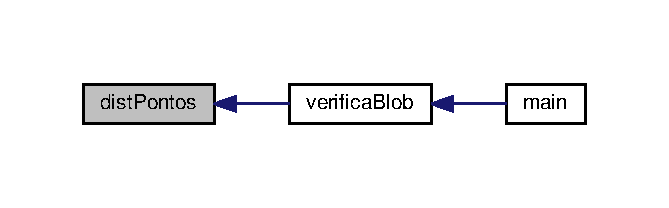
\includegraphics[width=321pt]{_main_8cpp_af393771749f2513a141d946bb885291b_icgraph}
\end{center}
\end{figure}
\mbox{\Hypertarget{_main_8cpp_afd251a63f3d03c2563a1f1dcf0ccb6f0}\label{_main_8cpp_afd251a63f3d03c2563a1f1dcf0ccb6f0}} 
\index{Main.\+cpp@{Main.\+cpp}!insere\+Blob@{insere\+Blob}}
\index{insere\+Blob@{insere\+Blob}!Main.\+cpp@{Main.\+cpp}}
\subsubsection{\texorpdfstring{insere\+Blob()}{insereBlob()}}
{\footnotesize\ttfamily void insere\+Blob (\begin{DoxyParamCaption}\item[{\hyperlink{class_blob}{Blob} \&}]{blob\+Atual,  }\item[{vector$<$ \hyperlink{class_blob}{Blob} $>$ \&}]{blobs\+Existentes,  }\item[{int \&}]{int\+Index }\end{DoxyParamCaption})}

Define os parâmetros do blob atual no vetor de blobs existentes Este é o diagrama das funções que utilizam esta função\+:
\nopagebreak
\begin{figure}[H]
\begin{center}
\leavevmode
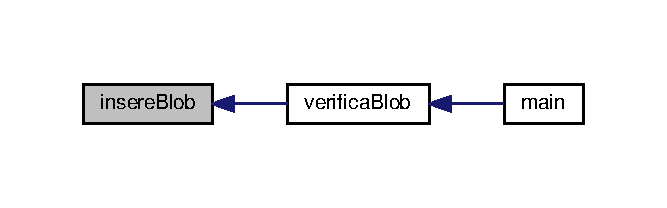
\includegraphics[width=320pt]{_main_8cpp_afd251a63f3d03c2563a1f1dcf0ccb6f0_icgraph}
\end{center}
\end{figure}
\mbox{\Hypertarget{_main_8cpp_a840291bc02cba5474a4cb46a9b9566fe}\label{_main_8cpp_a840291bc02cba5474a4cb46a9b9566fe}} 
\index{Main.\+cpp@{Main.\+cpp}!main@{main}}
\index{main@{main}!Main.\+cpp@{Main.\+cpp}}
\subsubsection{\texorpdfstring{main()}{main()}}
{\footnotesize\ttfamily int main (\begin{DoxyParamCaption}\item[{void}]{ }\end{DoxyParamCaption})}

Inicializa as linhas de referência da via direita e da esquerda, respectivamente

Caso não seja possível abrir o vídeo -\/ Erro

Caso o vídeo tenha apenas 1 frame (imagem) -\/ Erro

Captura 2 frames do vídeo

Controla a linha da direita

Controla a linha da esquerda

Inicializa os parâmetros para comparação dos frames

Converte os frames para a escala de cinza

Filtro de suavização gaussiano

Subtração da imagem

Limiarização

Elemento estruturante + Filtros morfológicos x2 (dilatação + erosão)

Define os contornos dos blobs

Define o envoltório convexo dos blobs

Verifica a linha da direita

Verifica a linha da esquerda

Via direita

Via esquerda

Passa o frame 2 para o frame 1

Verifica se o vídeo chegou ao fim Grafo de chamadas desta função\+:
\nopagebreak
\begin{figure}[H]
\begin{center}
\leavevmode
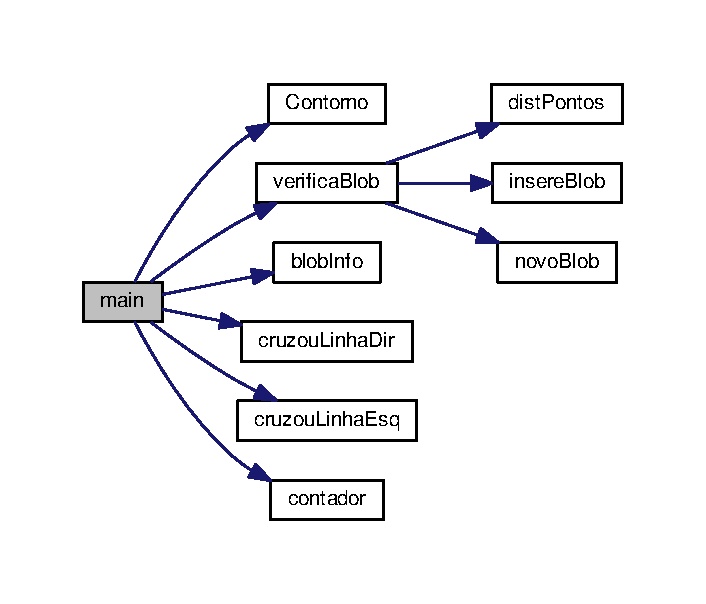
\includegraphics[width=339pt]{_main_8cpp_a840291bc02cba5474a4cb46a9b9566fe_cgraph}
\end{center}
\end{figure}
\mbox{\Hypertarget{_main_8cpp_a71c7b1ac1ca05b2e298a38fa1f7e58f8}\label{_main_8cpp_a71c7b1ac1ca05b2e298a38fa1f7e58f8}} 
\index{Main.\+cpp@{Main.\+cpp}!novo\+Blob@{novo\+Blob}}
\index{novo\+Blob@{novo\+Blob}!Main.\+cpp@{Main.\+cpp}}
\subsubsection{\texorpdfstring{novo\+Blob()}{novoBlob()}}
{\footnotesize\ttfamily void novo\+Blob (\begin{DoxyParamCaption}\item[{\hyperlink{class_blob}{Blob} \&}]{blob\+Atual,  }\item[{vector$<$ \hyperlink{class_blob}{Blob} $>$ \&}]{blobs\+Existentes }\end{DoxyParamCaption})}

Adiciona um novo blob no vetor de blobs existentes Este é o diagrama das funções que utilizam esta função\+:
\nopagebreak
\begin{figure}[H]
\begin{center}
\leavevmode
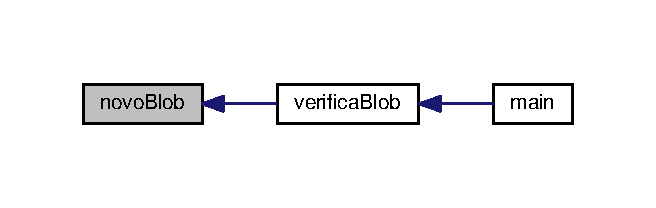
\includegraphics[width=315pt]{_main_8cpp_a71c7b1ac1ca05b2e298a38fa1f7e58f8_icgraph}
\end{center}
\end{figure}
\mbox{\Hypertarget{_main_8cpp_a3b43a4786c55005af285428e7c7ced87}\label{_main_8cpp_a3b43a4786c55005af285428e7c7ced87}} 
\index{Main.\+cpp@{Main.\+cpp}!verifica\+Blob@{verifica\+Blob}}
\index{verifica\+Blob@{verifica\+Blob}!Main.\+cpp@{Main.\+cpp}}
\subsubsection{\texorpdfstring{verifica\+Blob()}{verificaBlob()}}
{\footnotesize\ttfamily void verifica\+Blob (\begin{DoxyParamCaption}\item[{vector$<$ \hyperlink{class_blob}{Blob} $>$ \&}]{blobs\+Existentes,  }\item[{vector$<$ \hyperlink{class_blob}{Blob} $>$ \&}]{blobs\+Atuais }\end{DoxyParamCaption})}

Verifica se o blob atual já existe no vetor de blobs Inicializa as variáveis de distância Grafo de chamadas desta função\+:
\nopagebreak
\begin{figure}[H]
\begin{center}
\leavevmode
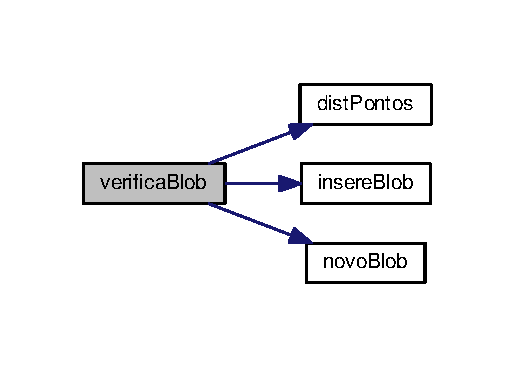
\includegraphics[width=247pt]{_main_8cpp_a3b43a4786c55005af285428e7c7ced87_cgraph}
\end{center}
\end{figure}
Este é o diagrama das funções que utilizam esta função\+:
\nopagebreak
\begin{figure}[H]
\begin{center}
\leavevmode
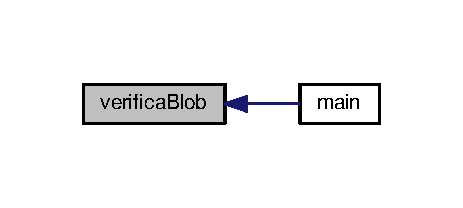
\includegraphics[width=222pt]{_main_8cpp_a3b43a4786c55005af285428e7c7ced87_icgraph}
\end{center}
\end{figure}


\subsection{Documentação das variáveis}
\mbox{\Hypertarget{_main_8cpp_a7b2cb89c87c76a1d832ef7ed097d9505}\label{_main_8cpp_a7b2cb89c87c76a1d832ef7ed097d9505}} 
\index{Main.\+cpp@{Main.\+cpp}!A\+M\+A\+R\+E\+LO@{A\+M\+A\+R\+E\+LO}}
\index{A\+M\+A\+R\+E\+LO@{A\+M\+A\+R\+E\+LO}!Main.\+cpp@{Main.\+cpp}}
\subsubsection{\texorpdfstring{A\+M\+A\+R\+E\+LO}{AMARELO}}
{\footnotesize\ttfamily const Scalar A\+M\+A\+R\+E\+LO = Scalar(0.\+0, 255.\+0, 255.\+0)}

Representação da cor Branca \mbox{\Hypertarget{_main_8cpp_a7c4a0519bc3e090ee4e3831391a9e018}\label{_main_8cpp_a7c4a0519bc3e090ee4e3831391a9e018}} 
\index{Main.\+cpp@{Main.\+cpp}!B\+R\+A\+N\+CO@{B\+R\+A\+N\+CO}}
\index{B\+R\+A\+N\+CO@{B\+R\+A\+N\+CO}!Main.\+cpp@{Main.\+cpp}}
\subsubsection{\texorpdfstring{B\+R\+A\+N\+CO}{BRANCO}}
{\footnotesize\ttfamily const Scalar B\+R\+A\+N\+CO = Scalar(255.\+0, 255.\+0, 255.\+0)}

Representação da cor Preta \mbox{\Hypertarget{_main_8cpp_a58d02c40e7b027e0b1ff6ce88c63280e}\label{_main_8cpp_a58d02c40e7b027e0b1ff6ce88c63280e}} 
\index{Main.\+cpp@{Main.\+cpp}!cont\+Dir@{cont\+Dir}}
\index{cont\+Dir@{cont\+Dir}!Main.\+cpp@{Main.\+cpp}}
\subsubsection{\texorpdfstring{cont\+Dir}{contDir}}
{\footnotesize\ttfamily int cont\+Dir = 0}

\mbox{\Hypertarget{_main_8cpp_a6bd1388b3554788f7d8d2019b2e00303}\label{_main_8cpp_a6bd1388b3554788f7d8d2019b2e00303}} 
\index{Main.\+cpp@{Main.\+cpp}!cont\+Esq@{cont\+Esq}}
\index{cont\+Esq@{cont\+Esq}!Main.\+cpp@{Main.\+cpp}}
\subsubsection{\texorpdfstring{cont\+Esq}{contEsq}}
{\footnotesize\ttfamily int cont\+Esq = 0}

Representação da cor Vermelha Inicializa os contadores de carros na parte esqueda e direita, respectivamente \mbox{\Hypertarget{_main_8cpp_a5f80550661781105dac995103754a262}\label{_main_8cpp_a5f80550661781105dac995103754a262}} 
\index{Main.\+cpp@{Main.\+cpp}!P\+R\+E\+TO@{P\+R\+E\+TO}}
\index{P\+R\+E\+TO@{P\+R\+E\+TO}!Main.\+cpp@{Main.\+cpp}}
\subsubsection{\texorpdfstring{P\+R\+E\+TO}{PRETO}}
{\footnotesize\ttfamily const Scalar P\+R\+E\+TO = Scalar(0.\+0, 0.\+0, 0.\+0)}

Define escalares de cores \mbox{\Hypertarget{_main_8cpp_aba06b79f5f073991c8a0afa7ebf9f534}\label{_main_8cpp_aba06b79f5f073991c8a0afa7ebf9f534}} 
\index{Main.\+cpp@{Main.\+cpp}!V\+E\+R\+DE@{V\+E\+R\+DE}}
\index{V\+E\+R\+DE@{V\+E\+R\+DE}!Main.\+cpp@{Main.\+cpp}}
\subsubsection{\texorpdfstring{V\+E\+R\+DE}{VERDE}}
{\footnotesize\ttfamily const Scalar V\+E\+R\+DE = Scalar(0.\+0, 200.\+0, 0.\+0)}

Representação da cor Amarela \mbox{\Hypertarget{_main_8cpp_a4d72d63fede13ee55603d480e2c28fd8}\label{_main_8cpp_a4d72d63fede13ee55603d480e2c28fd8}} 
\index{Main.\+cpp@{Main.\+cpp}!V\+E\+R\+M\+E\+L\+HO@{V\+E\+R\+M\+E\+L\+HO}}
\index{V\+E\+R\+M\+E\+L\+HO@{V\+E\+R\+M\+E\+L\+HO}!Main.\+cpp@{Main.\+cpp}}
\subsubsection{\texorpdfstring{V\+E\+R\+M\+E\+L\+HO}{VERMELHO}}
{\footnotesize\ttfamily const Scalar V\+E\+R\+M\+E\+L\+HO = Scalar(0.\+0, 0.\+0, 255.\+0)}

Representação da cor Verde 
\hypertarget{_r_e_a_d_m_e_8md}{}\section{Referência ao ficheiro R\+E\+A\+D\+M\+E.\+md}
\label{_r_e_a_d_m_e_8md}\index{R\+E\+A\+D\+M\+E.\+md@{R\+E\+A\+D\+M\+E.\+md}}

%--- End generated contents ---

% Index
\backmatter
\newpage
\phantomsection
\clearemptydoublepage
\addcontentsline{toc}{chapter}{Índice}
\printindex

\end{document}
